%!TEX program = latex
%!TEX encoding = UTF-8 Unicode

\documentclass{article}
\usepackage[letterpaper, top=0in, bottom=0in, left=0in, right=0in]{geometry}
\usepackage[utf8]{inputenc}
\usepackage[T1]{fontenc} 
\usepackage{concrete}  
\PassOptionsToPackage{dvipsnames,svgnames}{xcolor}
\usepackage[object=vectorian]{pgfornament}
\usepackage{lipsum}
\usetikzlibrary{shapes.multipart}
\usepackage{adjustbox}
\usepackage{setspace}

\usetikzlibrary{positioning,calc}
\usepackage{LobsterTwo}

\newcommand{\h}[1]{\textcolor{FireBrick}{#1}}
%\newcommand{\w}[1]{\textcolor[RGB]{218,165,32}{#1}}
\newcommand{\w}[1]{\textcolor[RGB]{225,223,0}{#1}}

\newfontfamily\carolyna[Path=fonts/]{Carolyna.otf}
\newfontfamily\imfell[Path=fonts/]{Optimus.ttf}

\begin{document}

\pagenumbering{gobble}% Remove page numbers (and reset to 1)
\begin{center} 

%\begin{tikzpicture}[color=black!60,transform shape,scale=1, 
%                     every node/.style={inner sep=0pt}]
\begin{tikzpicture}[xshift=0cm,yshift=-13.6cm,color=black!60,scale=1,overlay]
\node[minimum width=21.2cm,minimum height=27.7cm,fill=gray!0,inner sep=0pt](vecbox){}; 
\node[anchor=north west] at (vecbox.north west){\pgfornament[color=MidnightBlue,width=2cm]{39}};
\node[anchor=north east] at (vecbox.north east){\pgfornament[color=MidnightBlue,width=2cm,symmetry=v]{39}};
\node[anchor=south west] at (vecbox.south west){\pgfornament[color=MidnightBlue,width=2cm,symmetry=h]{39}};
\node[anchor=south east] at (vecbox.south east){\pgfornament[color=MidnightBlue,width=2cm,symmetry=c]{39}};
 \node[anchor=north,yshift=2pt] at (vecbox.north){\pgfornament[width=16cm,symmetry=h]{88}};
 \node[anchor=south,yshift=-2pt] at (vecbox.south){\pgfornament[width=16cm]{88}};
 \node[anchor=north,rotate=90,yshift=2pt]  at (vecbox.west){\pgfornament[width=23cm,symmetry=h]{88}};
 \node[anchor=north,rotate=-90,yshift=2pt] at (vecbox.east){\pgfornament[width=23cm,symmetry=h]{88}};

 \foreach \y in {-7,-6,-5,-4,-3,-2,-1,0,1,2,3,4,5,6,7}
    \draw[black!40] (-9cm,1.6*\y cm) -- (9cm,1.6*\y cm);
\end{tikzpicture} 

\end{center}

\begin{center}
\adjustbox{padding*=0ex 0ex 0ex 0ex,margin*=20ex 0ex 0ex 40ex}{
\begin{minipage}[b]{0.8\textwidth}
	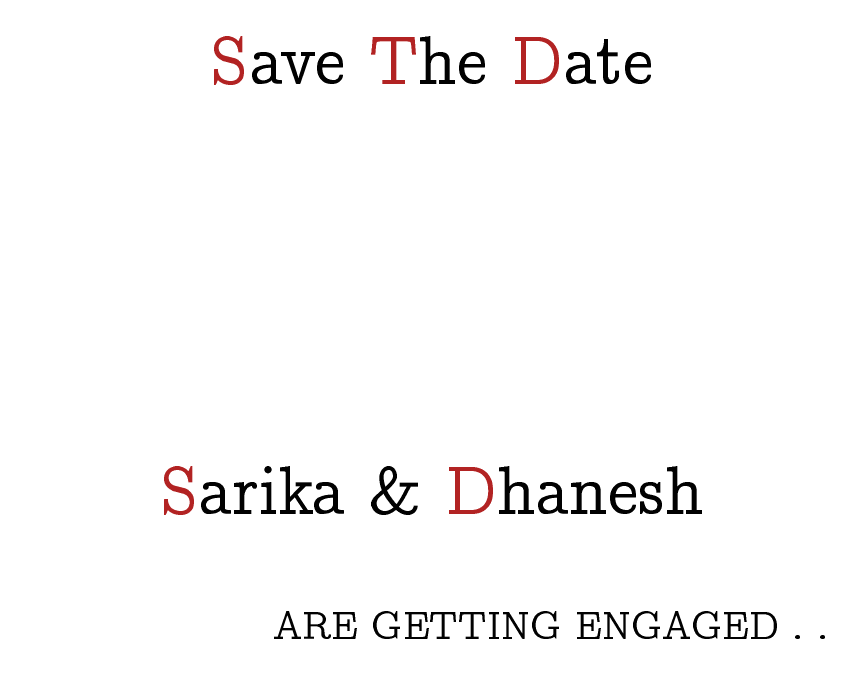
\begin{tikzpicture}
        \node(x1) at (0, 0) {\LobsterTwo \fontsize{36}{38}\selectfont \h{S}ave \h{T}he \h{D}ate};
        \node(x2) [below = 4.6cm of x1] {\centering \carolyna \fontsize{50}{50}\selectfont \h{S}arika \& \h{D}hanesh};
        \node(x3) [below = 1cm of x2]{\imfell \centering \fontsize{15}{15}\selectfont \centering \hspace{3cm}\uppercase{are getting engaged . .}};
    \end{tikzpicture}
\end{minipage}
}
\end{center}


\end{document}